\scanpage{32}\mspage{31}
% Provisional main-reader proposal, before comparison of the three reports.
% @ top, continuation
Si $A\in F\setminus G$, $A\cap B$ est réunion de strates de $F$. \deleted{Reste} reste \unsure{à|:} voir que une strate 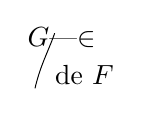
\begin{tikzpicture}[baseline=(de.base)]
\node[anchor=base west,inner sep=0pt] at (-.15,.48) {\inserted{\unsure{$G$|$\in$}}};
\node[anchor=base west,inner sep=0pt] (de) at (.2,0) {de $F$};
\draw[line width=.35pt] (-.05,-.05)..controls(.02,.25)and(.12,.42)..(.2,.65);
\end{tikzpicture} est réunion de strates de $F'$. Soit $A$ cette strate de $F$. \deleted{On}
\[
 \deleted{A=\bigcup_{\substack{B\in F\\B\leq F}}B^\circ}
\]
Si $A\notin G'$, alors $A\in F\mathbin{\underset{\begin{tikzpicture}[x=1ex,y=1ex,baseline=0pt]
\draw[line width=.45pt,line cap=round] (.30,.65) .. controls (.38,.36) and (.12,.18) .. (0,0);
\draw[line width=.45pt,line cap=round] (.16,.45)--(0,0)--(.20,0);
\end{tikzpicture}}{\setminus}}G'\subset F'$, et on gagne. Si $A\in G$, alors (comme $G'\preceq G$) $A$ est réunion de strates de $G'$, qui sont des strates de $F'$, et on gagne encore.

% @ left, oblique
\margin{Ultra faux}
% @ heading, subdivision and chacune interlinear
\figure{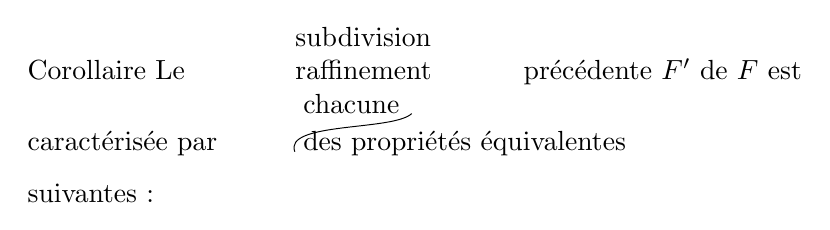
\begin{tikzpicture}[x=1cm,y=1cm]
\node[anchor=base west,inner sep=0pt] at (0,0) {\uline{Corollaire} Le};
\node[anchor=base west,inner sep=0pt] (oldnoun) at (3.4,0) {\deleted{raffinement}};
\node[anchor=base west,inner sep=0pt] at (3.4,.42) {\inserted{subdivision}};
\node[anchor=base west,inner sep=0pt] at (6.3,0) {précédente $F'$ de $F$ est};
\node[anchor=base west,inner sep=0pt] at (0,-.9) {caractérisée par};
\node[anchor=base west,inner sep=0pt] (chacune) at (3.5,-.42) {\inserted{chacune}};
\node[anchor=base west,inner sep=0pt] (des) at (3.5,-.9) {des propriétés équivalentes};
\draw[line width=.35pt] ([xshift=-.1cm,yshift=-.1cm]des.west)..controls(3.25,-.53)and(4.65,-.65)..([xshift=.15cm]chacune.south east);
\node[anchor=base west,inner sep=0pt] at (0,-1.55) {suivantes~:};
\end{tikzpicture}}

% @ whole a) crossed by two large diagonals; maximal also locally cancelled
\figure{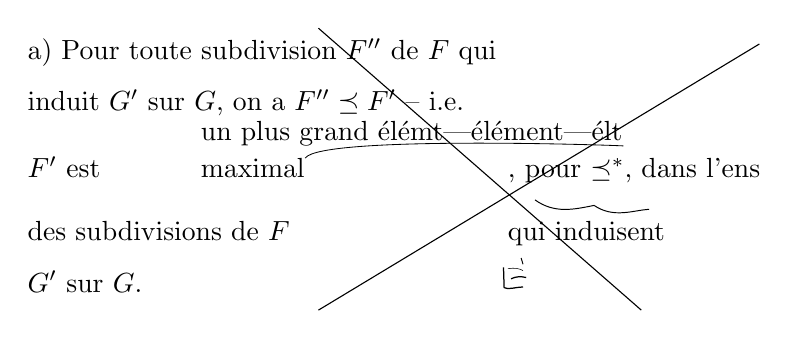
\begin{tikzpicture}
\node[anchor=base west,inner sep=0pt] at (0,0) {\deleted{a) Pour toute subdivision $F''$ de $F$ qui}};
\node[anchor=base west,inner sep=0pt] at (0,-.65) {\deleted{induit $G'$ sur $G$, on a $F''\preceq F'$ -- i.e.}};
\node[anchor=base west,inner sep=0pt] at (0,-1.5) {\deleted{$F'$ est}};
\node[anchor=base west,inner sep=0pt] (oldmax) at (2.2,-1.5) {\deleted{\uline{maximal}}};
\node[anchor=base west,inner sep=0pt] (newmax) at (2.2,-1.02) {\deleted{\inserted{un plus grand \unsure{élémt|élément|élt}}}};
\node[anchor=base west,inner sep=0pt] at (6.1,-1.5) {\deleted{, pour $\preceq^{*}$, dans l'ens}};
\draw[line width=.3pt] (oldmax.north east)..controls([xshift=.2cm,yshift=.3cm]oldmax.north east)and([xshift=.2cm]newmax.south east)..(newmax.south east);
\draw[line width=.35pt] (6.45,-1.78)..controls(6.7,-1.96)and(6.95,-1.9)..(7.2,-1.85)..controls(7.45,-2.02)and(7.7,-1.91)..(7.9,-1.9);
\node[anchor=base west,inner sep=0pt] at (0,-2.3) {\deleted{des subdivisions de $F$}};
\node[anchor=base west,inner sep=0pt] at (6.1,-2.3) {\deleted{qui induisent}};
\node[anchor=base west,inner sep=0pt] at (0,-2.95) {\deleted{$G'$ sur $G$.}};
% Unidentified angular mark directly below qui, inside the crossed block.
\begin{scope}[shift={(6.05,-2.91)},scale=.8]
\draw[line width=.45pt] (0,.34)--(.01,.02)..controls(.07,-.02)and(.20,.03)..(.31,.03);
\draw[line width=.45pt] (.12,.16)..controls(.21,.20)and(.27,.20)..(.36,.18);
\draw[line width=.2pt] (.07,.32)..controls(.18,.34)and(.26,.32)..(.31,.29);
\draw[line width=.35pt] (.28,.49)--(.31,.39);
\end{scope}
\draw[line width=.4pt] (3.7,.4)--(7.8,-3.18);
\draw[line width=.4pt] (3.7,-3.18)--(9.3,.2);
\end{tikzpicture}}
% @ oblique starred gloss
\margin{$*$ ou pour $\ll$, \unsure{cela|cel} revient au $=$ parmi des subdivisions d'une $=$ $F$}
% @ long oblique note, traversed by curved pen stroke
\margin{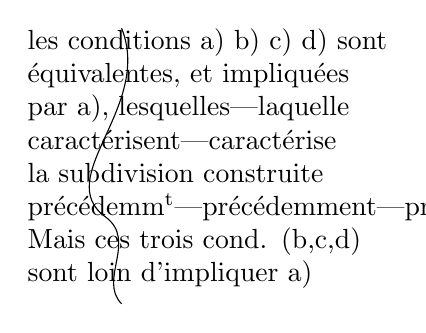
\begin{tikzpicture}
% The outer doubt concerns cancellation state, not the securely read words.
\node[anchor=north west,text width=4.7cm,inner sep=0pt] (note) at (0,0) {\unsure{\deleted{les conditions \deleted{\unsure{a)}} b) c) d) sont équivalentes, \unsure{et} \uline{impliquées} par a), \unsure{lesquelles|laquelle} \unsure{caractérisent|caractérise} la subdivision construite \unsure{précédemm\textsuperscript{t}|précédemment|précédemment\textsuperscript{\#}}. Mais ces trois \unsure{cond.} (b,c,d) sont \unsure{loin} d'impliquer a)}}};
\draw[line width=.4pt] ([xshift=1.2cm]note.north west)..controls(1.6,-1.0)and(.3,-1.9)..(1.0,-2.4)..controls(1.4,-2.7)and(.9,-3.2)..(1.2,-3.5);
\end{tikzpicture}}
b) L'application can. associée à $F'\preceq F$
\[
 \varphi:F'\longrightarrow F
\]
induit une bijection
\[
 F'\setminus G'\xrightarrow{\sim}F\setminus G.
\]
% @ right note, left vertical stroke
\margin{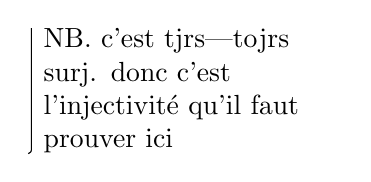
\begin{tikzpicture}
\node[anchor=north west,text width=3.8cm,inner sep=0pt] (nb) at (0,0) {NB. c'est \unsure{tjrs|tojrs} surj. donc c'est l'\uline{injectivité} qu'il faut prouver ici};
\draw[line width=.4pt] ([xshift=-.15cm]nb.north west)--([xshift=-.15cm,yshift=.08cm]nb.south west)..controls([xshift=-.15cm,yshift=.02cm]nb.south west)..([xshift=-.19cm]nb.south west);
\end{tikzpicture}}
% @ c): new sentence above the complete cancelled baseline, shared final de F'
c) \deleted{Les strates ouvertes de $F'$ qui ne sont} \inserted{$\forall A\in F\setminus G$, $A^\circ$ est une strate ouverte} de $F'$.
d) $F'\supset F\setminus G$, i.e. $\forall A\in F\setminus G$, on a $A\in F'$.
% @ foot: one On only
\uline{Dém} On va prouver p. ex
\[
 \text{d)}\Longrightarrow\text{b)}\Longrightarrow\text{c)}\Longrightarrow\text{a)}\Longrightarrow\text{d)}
\]
\deleted{\uline{Dém}} $\text{d)}\Rightarrow\text{b)}$ Si $(F\setminus G)\subset F'$, alors $\varphi\mid F\setminus G$ est l'\deleted{\unsure{identité}}\unsure{inclusion} \deleted{(trivial)} \inserted{can. $F\setminus G\hookrightarrow F$}, \deleted{donc} donc il reste à prouver
\[
 F\setminus G=F'\setminus G'.
\]
